  GNU nano 7.2                                                            maths.tex
\documentclass[12pt,a4paper]{article}
\usepackage{amsmath}
\usepackage{graphicx}
\usepackage{geometry}
\usepackage{multicol}
\geometry{margin=1in}

\begin{document}

% ---------- CUSTOM TITLE ----------
\begin{center}
\begin{minipage}{0.2\textwidth}
    
\includegraphics[width=\linewidth]{iiit_logo.png} 
\end{minipage}
\hfill
\begin{minipage}{0.75\textwidth}
    \centering
    {\Large \textbf{MATHEMATICS}}\\[1ex]
    \textbf{Name: Varshini G N} \\[0.5ex]
    ID:COMETFWC031\\
    \textbf{Date:} \today
\end{minipage}
\end{center}

\vspace{1em}
\title{CBSE Maths Question Paper 2016}
\hrule
\vspace{1em}


\begin{center}
\textbf{1 A} \\
\textit{question numbers 1 to 4 carry 1 mark each.}
\end{center}

\begin{multicols}{2}

\begin{enumerate}

    \item In Fig., PQ is a tangent at point C to a circle with centre O. If AB is a diameter and $\angle CAB = 30^\circ$, find $\angle PCA$.\\
    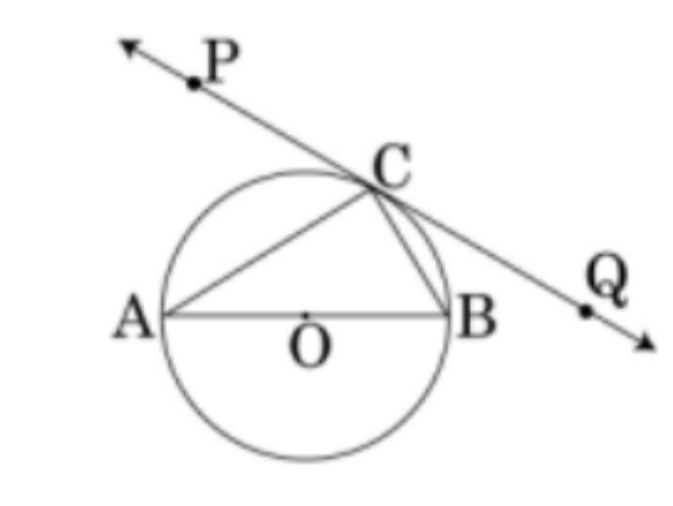
\includegraphics[width=\linewidth]{circle_diagram.png}

    \item For what value of $k$ will $k+9$, $2k-1$ and $2k+7$ be the consecutive terms of an A.P.?

    \item A ladder, leaning against a wall, makes an angle of $60^\circ$ with the horizontal. If the foot of the ladder is 2.5 m away from the wall, fi>

    \item A card is drawn at random from a well shuffled pack of 52 playing cards. Find the probability of getting neither a red card nor a queen.

    \columnbreak

    \begin{center}
    \textbf{2 B} \\
    \textit{Question numbers 5 to 10 carry 2 marks each.}
    \end{center}

    \item If $-5$ is a root of the quadratic equation $2x^2 + px - 15 = 0$ and the quadratic equation $p(x^2 + x) + k = 0$ has equal roots, find the va>

    \item Let P and Q be the points of trisection of the line segment joining the points $A(2, -2)$ and $B(7, 4)$ such that P is nearer to A. Find the >

    \item In Fig., a quadrilateral ABCD is drawn to circumscribe a circle, with centre O, in such a way that the sides AB, BC, CD and DA touch the circ>
    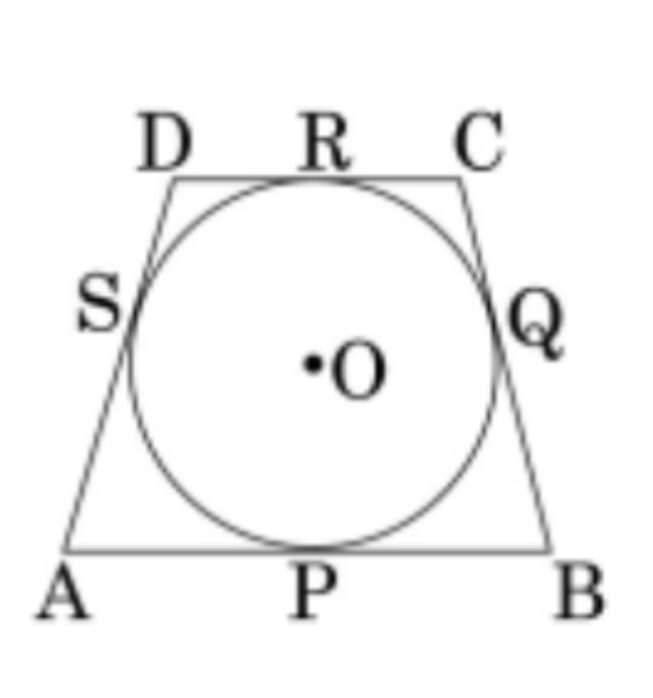
\includegraphics[width=\linewidth]{quadrilateral_diagram.png}

    \item Prove that the points (3, 0), (6, 4) and (-1, 3) are the vertices of a right angled isosceles triangle.

    \item The 4th term of an A.P. is zero. Prove that the 25th term of the A.P. is three times its 11th term.

    \item In Fig., from an external point P, two tangents PT and PS are drawn to a circle with centre O and radius r. If $OP = 2r$, show that $\angle O>
\end{enumerate}

\end{multicols}

\end{document}






